\documentclass[12pt, a4paper]{article}
\usepackage[utf8]{vietnam}
\usepackage{mathptmx}

% lib component
\usepackage{tikz}
\usepackage{amsmath}
\usepackage{tikz-cd}
\usepackage{amsfonts}
\usepackage{amssymb}
\usepackage{graphics}
\usepackage{array}
\usepackage{cases}
\usepackage{mdframed}
\usepackage{fancybox}
\usepackage{enumerate}
\usepackage{diagbox}
\usepackage{soul}
\usepackage{caption}
\usepackage{floatrow}
\usepackage{scrextend}
\usepackage{tikz} 
\usepackage{scrextend}
\usepackage{fancyhdr}
\usepackage{amsmath}
\usepackage[thref,thmmarks,standard,amsmath,hyperref]{ntheorem}
\usepackage{multicol}
% ----- Theorem:
%\theoremstyle{definition}
%\newtheorem{definition}{Định nghĩa}[section]

%\theoremstyle{definition}
%\newtheorem{theorem}{Định lý}[section]
%\newtheorem*{remark}{Nhận xét}
%\newtheorem{vd}{Ví dụ}[section]
%\newtheorem{bt}{Bài tập}[section]
%\newtheorem{tc}{Tính chất}[section]
%\newtheorem{md}{Mệnh đề}[section]
%\newtheorem{cy}{Chú ý}[section]
%\newtheorem{nx}{Nhận xét}[section]

% ----- Constant:
% Thông tin về đồ án
\def\author{Nguyễn Bùi Nam Trường}
\def\mssv{20185418}
\def\SCHOOL{TRƯỜNG ĐẠI HỌC BÁCH KHOA HÀ NỘI}
\def\school{Trường Đại học Bách Khoa Hà Nội}
\def\INSTITUTE{VIỆN TOÁN ỨNG DỤNG VÀ TIN HỌC}
\def\institute{Viện Toán ứng dụng và Tin học}


\def\instructor{Nguyễn Huy Trường}
\def\INSTRUCTOR{TS. Nguyễn Huy Trường}

\def\PROJECT{LẬP TRÌNH ANDROID}
\def\project{Lập trình Android}
\def\projects{Lập trình Android với React Native}

% ----- Style:
\usepackage{xcolor}
\usepackage[left=3.5cm, right=2cm, top=3.5cm, bottom=3cm]{geometry}
\usepackage[colorlinks=true, allcolors=black, unicode]{hyperref}
\changefontsizes[18pt]{13pt}
\setlength{\parindent}{0.6cm}
\usepackage{indentfirst}
\setlength{\parskip}{2pt}
\renewcommand{\baselinestretch}{1.4}
\setlength{\baselineskip}{18truept}
\renewcommand{\headrulewidth}{0.5pt}
\renewcommand{\footrulewidth}{0.5pt}
\usepackage[]{hyperref}

% ----- Format:
\pagestyle{fancy}
\fancyhf{}
\usepackage{enumerate}
\usepackage{enumitem}
\lhead{\normalsize \projects}
\rhead{\normalsize \project}
\lfoot{\normalsize \author - \mssv}
\rfoot{Trang \thepage}
% \renewcommand\thesection{Chương \Roman{section}}
% \renewcommand\thesubsection{\arabic{subsection}}

% ----- Mục lục:
\newcommand{\nocontentsline}[3]{}
\newcommand{\tocless}[2]{\bgroup\let\addcontentsline=\nocontentsline#1{#2}\egroup}

% ------------------------------------------------------- %

\begin{document}
    	% ----- Trang bìa: Hoàn thành
        \begin{titlepage}
	\begin{tikzpicture}[remember picture,overlay,inner sep=0,outer sep=0]
		\draw[blue!70!black,line width=5pt] 
		([xshift=-2cm,yshift=-2cm]current page.north east) coordinate (A)--
		([xshift=2cm,yshift=-2cm]current page.north west) coordinate(B)--
		([xshift=2cm,yshift=2cm]current page.south west) coordinate (C)--
		([xshift=-2cm,yshift=2cm]current page.south east) coordinate(D)--cycle;
		
		\draw ([yshift=0.5cm,xshift=-0.5cm]A)-- ([yshift=0.5cm,xshift=0.5cm]B)-- ([yshift=-0.5cm,xshift=0.5cm]B) --([yshift=-0.5cm,xshift=-0.5cm]B)--([yshift=0.5cm,xshift=-0.5cm]C)--([yshift=0.5cm,xshift=0.5cm]C)--([yshift=-0.5cm,xshift=0.5cm]C)-- ([yshift=-0.5cm,xshift=-0.5cm]D)--([yshift=0.5cm,xshift=-0.5cm]D)--([yshift=0.5cm,xshift=0.5cm]D)--([yshift=-0.5cm,xshift=0.5cm]A)--([yshift=-0.5cm,xshift=-0.5cm]A)--([yshift=0.5cm,xshift=-0.5cm]A);
		
		
		\draw ([yshift=-0.3cm,xshift=0.3cm]A)-- ([yshift=-0.3cm,xshift=-0.3cm]B)--
		([yshift=0.3cm,xshift=-0.3cm]B) --([yshift=0.3cm,xshift=0.3cm]B)--([yshift=-0.3cm,xshift=0.3cm]C)--([yshift=-0.3cm,xshift=-0.3cm]C)--([yshift=0.3cm,xshift=-0.3cm]C)-- ([yshift=0.3cm,xshift=0.3cm]D)--([yshift=-0.3cm,xshift=0.3cm]D)--([yshift=-0.3cm,xshift=-0.3cm]D)--([yshift=0.3cm,xshift=-0.3cm]A)--([yshift=0.3cm,xshift=0.3cm]A)--([yshift=-0.3cm,xshift=0.3cm]A);
	\end{tikzpicture}
	\begin{center}
		\begin{large}
			\textbf{\SCHOOL}\\
			\textbf{\INSTITUTE}\\
		\end{large}
		\centerline{--------------------o0o--------------------}
		\vspace{0.5cm}
		\includegraphics[scale=0.6]{images/logo.jpg}\\
		\vspace{0.5cm}
		{\fontsize{28pt}{1}\selectfont \textbf{\PROJECT}}\\
		\vspace{0.5cm}
		{\fontsize{16pt}{1}\selectfont \textbf{ĐỒ ÁN II}}\\
		{\fontsize{13pt}{1}\selectfont \textbf{Chuyên ngành: TOÁN TIN}}\\
		{\fontsize{13pt}{1}\selectfont \textbf{\textcolor{red}{Chuyên sâu: \projects}}}
	\end{center}
	\vspace{0.5cm}
	\begin{center}
		\begin{tabular}{ll}
			Giảng viên hướng dẫn & : \textbf{\INSTRUCTOR}\\
			Nhóm sinh viên thực hiện & : \textbf{\author}\\
			MSSV & : \textbf{20185418}\\
		\end{tabular}
	\end{center}
	\vspace{0.5cm}
	\begin{center}
		{\bf HÀ NỘI, tháng ../2022}
	\end{center}
\end{titlepage}
	
        % ----- Nhận xét của Giảng viên: Hoàn thành
        \thisfancypage{
	\fbox
}{}
\newpage
\begin{center}
	\textbf{NHẬN XÉT CỦA GIẢNG VIÊN HƯỚNG DẪN}
\end{center}
\begin{enumerate}
	\item [{\bfseries 1.}]{\bfseries Mục đích và nội dung của đồ án:}
	\begin{enumerate}
		\item[-] 
		\item[-] 
		\item[-] 
	\end{enumerate}
	\item [{\bfseries 2.}] {\bfseries Kết quả đạt được} 
	\begin{enumerate}
		\item[-] 
		\item[-] 
		\item[-] 
	\end{enumerate}
	\item [{\bfseries 3.}]{\bfseries Ý thức làm việc của sinh viên:}
	\begin{enumerate}
		\item[-]
		\item[-]
		\item[-]
	\end{enumerate}
	\begin{flushright}
		\begin{tabular}{lc}
			& \textit{Hà Nội, ngày .. tháng .. năm 2022}\\
			& Giảng viên\\
			& \\
			& \textbf{\INSTRUCTOR}\\
		\end{tabular}
	\end{flushright}
\end{enumerate}
\newpage
        
        % ----- Lời nói đầu:
        \newpage
\section*{\centering Lời nói đầu}
\addcontentsline{toc}{section}{Lời nói đầu}
% Giới thiệu về lập trình android
Ngày nay, cùng với sự phát triển mạnh mẽ của lĩnh vực Công nghệ thông tin, có rất nhiều công ty công nghệ lớn nhỏ được sinh ra. Các công ty đó vẫn liên tục phát triển và cải tiến để phục vụ cuộc sống con người và xã hội. Một trong những sản phẩm phổ biến và dần trở nên không thể thiêu đối với người dùng là điện thoại di động. Tính đến tháng 6/2020, trong thế giới rộng lớn của điện thoại di đọng, hệ điều hành Android đã chiểm 74.4\% thị phần toàn cầu và 60.8\% thị phần Việt Nam. Với sức bao phủ và ảnh hưởng lớn như vậy, việc tìm hiểu về hệ điều hành này là qua trong đối với những người học tập và làm việc trong lĩnh vực công nghệ.
% Giới thiệu về React Native
Cũng như sự phổ biến của Android trong thế giới điện thoại di động, các phần mềm được xây dựng dựa trên công cụ React Native cũng dần trở nên phổ biến và được ưa chuộng đối với các nhà phát triển ứng dụng.
% Chọn đề tài
Sau một thời gian học tập tại trường Đại học Bách Khoa Hà Nội, viện Toán ứng dụng và Tin học, em đã tích lũy được vốn kiến thức nhất định và đang thực hiện học phần Đồ Án II. Được sự đồng ý của nhà trường và các thầy cô trong viện, em được giao đề tài cho đồ án: \textit{"Tìm hiểu về Lập trình Android với React Native"}.
% Tóm tắt nội dung đồ án
Bài Đồ án này gồm ba chương:

Chương 1: Giới thiệu về Android.

Chương 2: Giới thiệu về React Native.

Chương 2: Xây dựng ứng dụng Android với React Native.

% Lời cảm ơn
Bằng sự cố gắng nỗ lực của bản thân và đặc biệt là sự giúp đỡ tận tình, chu đáo của thầy \instructor, em đã hoàn thành đồ án đúng thời hạn. Do thời gian làm đồ án có hạn và trình độ còn nhiều hạn chế nên không thể tránh khỏi những thiếu sót. Em rất mong nhận được sự đóng góp ý kiến của các thầy cô cũng như là của các bạn sinh viên để bài đồ án này hoàn thiện hơn nữa. Em xin chân thành cảm ơn thầy \instructor, các thầy cô trong viện Toán ứng dụng và Tin học trường Đại học Bách Khoa Hà Nội đã tạo điều kiện giúp đỡ em trong thời gian qua.

\begin{flushright}
	\begin{tabular}{rc}
		& Hà Nội, ngày .. tháng .. năm 2022 \\
		& Sinh viên thực hiện \\	
		\\
		& Nguyễn Bùi Nam Trường \\
	\end{tabular}
\end{flushright}
\newpage
        
        % ----- Mục lục:
        \tableofcontents	
        
        % ----- Kí hiệu và từ viết tắt:
        % \begin{titlepage}
	\begin{tikzpicture}[remember picture,overlay,inner sep=0,outer sep=0]
		\draw[blue!70!black,line width=5pt] 
		([xshift=-2cm,yshift=-2cm]current page.north east) coordinate (A)--
		([xshift=2cm,yshift=-2cm]current page.north west) coordinate(B)--
		([xshift=2cm,yshift=2cm]current page.south west) coordinate (C)--
		([xshift=-2cm,yshift=2cm]current page.south east) coordinate(D)--cycle;
		
		\draw ([yshift=0.5cm,xshift=-0.5cm]A)-- ([yshift=0.5cm,xshift=0.5cm]B)-- ([yshift=-0.5cm,xshift=0.5cm]B) --([yshift=-0.5cm,xshift=-0.5cm]B)--([yshift=0.5cm,xshift=-0.5cm]C)--([yshift=0.5cm,xshift=0.5cm]C)--([yshift=-0.5cm,xshift=0.5cm]C)-- ([yshift=-0.5cm,xshift=-0.5cm]D)--([yshift=0.5cm,xshift=-0.5cm]D)--([yshift=0.5cm,xshift=0.5cm]D)--([yshift=-0.5cm,xshift=0.5cm]A)--([yshift=-0.5cm,xshift=-0.5cm]A)--([yshift=0.5cm,xshift=-0.5cm]A);
		
		
		\draw ([yshift=-0.3cm,xshift=0.3cm]A)-- ([yshift=-0.3cm,xshift=-0.3cm]B)--
		([yshift=0.3cm,xshift=-0.3cm]B) --([yshift=0.3cm,xshift=0.3cm]B)--([yshift=-0.3cm,xshift=0.3cm]C)--([yshift=-0.3cm,xshift=-0.3cm]C)--([yshift=0.3cm,xshift=-0.3cm]C)-- ([yshift=0.3cm,xshift=0.3cm]D)--([yshift=-0.3cm,xshift=0.3cm]D)--([yshift=-0.3cm,xshift=-0.3cm]D)--([yshift=0.3cm,xshift=-0.3cm]A)--([yshift=0.3cm,xshift=0.3cm]A)--([yshift=-0.3cm,xshift=0.3cm]A);
	\end{tikzpicture}
	\begin{center}
		\begin{large}
			\textbf{\SCHOOL}\\
			\textbf{\INSTITUTE}\\
		\end{large}
		\centerline{--------------------o0o--------------------}
		\vspace{0.5cm}
		\includegraphics[scale=0.6]{images/logo.jpg}\\
		\vspace{0.5cm}
		{\fontsize{28pt}{1}\selectfont \textbf{\PROJECT}}\\
		\vspace{0.5cm}
		{\fontsize{16pt}{1}\selectfont \textbf{ĐỒ ÁN II}}\\
		{\fontsize{13pt}{1}\selectfont \textbf{Chuyên ngành: TOÁN TIN}}\\
		{\fontsize{13pt}{1}\selectfont \textbf{\textcolor{red}{Chuyên sâu: \projects}}}
	\end{center}
	\vspace{0.5cm}
	\begin{center}
		\begin{tabular}{ll}
			Giảng viên hướng dẫn & : \textbf{\INSTRUCTOR}\\
			Nhóm sinh viên thực hiện & : \textbf{\author}\\
			MSSV & : \textbf{20185418}\\
		\end{tabular}
	\end{center}
	\vspace{0.5cm}
	\begin{center}
		{\bf HÀ NỘI, tháng ../2022}
	\end{center}
\end{titlepage}
    
        % ----- Nội dung chính
        % Chương 1: Giới thiệu về Android
%     1.1 Khái niệm về Android
%     1.2 Kiến trúc của Android
% Chương 2: Môi trường lập trình Android
% Chương 3: Giới thiệu về React và ReactNative


\newpage
% ----- Chương 1:
\section{Giới thiệu về Android}

\subsection{Khái niệm về Android}
Trước hết, Hệ điều hành (Operating System - OS) là phần mềm hệ thống quản lý phần cứng máy tính, phần mềm và cung cấp các dịch vụ chung cho các chương trình máy tính.
Android là hệ điều hành dựa trên mã nguồn mở Linux OS cho các thiết bị di động và các thiết bị thông minh như máy tính bảng, laptop, netbook, smartbook, TV thông minh(Google TV),\dots Hiện nay, một số hệ điều hành cho thiết bị di động: Android, OS X (iPhone), Windows Mobile, Symbian,\dots Tuy nhiên, hệ điều hành được sử dụng nhiều nhất là Android và OS X.

% Điểm nổi bật của Android
Ngay từ khi ra mắt, Android đã gây ấn tượng mạnh khi đây là đứa con của Goodle sử dụng giấy phép mã nguồn mở. Android là sản phẩm kết tinh từ ý tưởng của Khối Liên minh thiết bị cầm tay mở do Google dẫn đầu, gồm 34 thành viên với các công ty hàng đầu về công nghệ và di động toàn cầu như Qualcomm, Intel, Motorola, Texas Instruments và LG Electronics, các nhà mạng như T-Mobile, Sprint Nextel, NTT DoCoMo và China Mobile.

% Đặc tính mở của Android
Với đặc tính "mở", Android cho phép các nhà phát triển có thể sử dụng miễn phí bộ Kit Android Software Development để xây dựng các ứng dụng của mình. Ví dụ, một ứng dụng có thể gọi bất kì chức năng lõi của điện thoại như thực hiện gọi, gửi tin nhắn, sử dụng máy ảnh,\dots Điều này thực sự thu hút các nhà phát triển sáng tạo ra các phần mềm hấp dẫn, từ đó tạo ra một cộng đồng phát triển lớn - là nguyên nhân đến sự phổ biến của Android như hiện nay.

\subsection{Kiến trúc của Android}
Để bắt đầu lập trình với Android, chúng ta cần nghiên cứu qua bản thân HĐH Android, chúng ta không cần hiểu quá chi tiết, nhưng trước hết là cần có cái nhìn chung và toàn diện nhất về Android.

Android Platform bao gồm đầy đủ các tính năng HĐH Android, các ứng dụng và các tâng trung gian để nhà phá triển có thể mở rộng, tùy chỉnh thêm theo nhu cầu của họ. Có 4 tầng cơ bản trong HĐH Android: Linux Kernel, Native Libraries, Android Runtime, Application Framework,\dots Các tầng làm việc có sự liên kết với nhau.
\begin{enumerate}
    \item{\textit{Tầng Linux Kernel:}}
    Đây là tầng nhân của HĐH Android, Linux Kernel giúp hệ điều hành có thể giao tiếp với phần cứng của thiết bị như: camera,  USB, Wifi, Bluetooth, Display, Power Management,\dots  Linux Kernel chịu trách nhiệm cho các trình điều khiển thiết bị, quản lý nguồn điện, quản lý bộ nhớ, quản lý thiết bị và truy cập tài nguyên. Kernel hoạt động như một lớp trừu tượng giữa phần cứng và phần mềm còn lại của hệ thống.
    \item{\textit{Native Libraries:}}
    Native Libraries là tập hợp của nhiều thư viện như WebKit, OpenGL, FreeType, SQLite, Media, SSL,\dots 
    \item{\textit{Tầng Android Runtime:}}
    Android Runtime cung cấp một thành phần quan trọng được gọi là DVM (Dalvik Virtual Machine - máy ảo) có trách nhiệm chạy ứng dụng android.
    DVM thực thi các file có định dạng .dex (Dalvik Excutable), định dạng này là định dạng được tối ưu hóa về bộ nhớ.
    \newline
    DVM có phần tương tự như JVM (Java Virtual Machine) nhưng được tối ưu hóa cho các thiết bị di động như tiêu thụ ít bộ nhớ hơn và tăng hiệu suất hoạt động tốt hơn.
    \item{\textit{Tầng Application Framework:}}
    Application Framework bao gồm tập hợp những API cho phép các nhà phát triển ứng dụng được phép sử dụng các dịch vụ này trong các ứng dụng của họ.
\end{enumerate}
Ở góc độ người dùng, ta có thêm tầng Application - là các ứng dụng do nhà phát triển ứng dụng viết. Dưới đây là sơ đồ tương quan liên kết giữa các tầng:
\newline
\begin{figure}[!ht]
    \centering
    \includegraphics[scale=0.5]{images/android-flatform.jpg}
    \caption{Sơ đồ tương quan liên kết giữa các tầng}
\end{figure}



% ----- Chương 2:
\section{Giới thiệu về React Native}

\subsection{Giới thiệu}
React Native là một Framework, do công ty Công nghệ Meta (trước đây là Facebook) phát triển, nhằm giải quyết vấn đề về hiệu năng và việc phải sử dụng nhiều ngôn ngữ native trên nền tảng di động.

React Native cho phép xây dựng và phát triển ứng dụng native đa nền tảng một cách dễ dàng, khác với HTML5 App, Mobile Web App, Hybrid App. Mục đích khi tạo ra React Native là khắc phục các điểm yếu của ứng dụng web, giúp cho nhà lập trình tiết kiệm thời gian, công sức bởi sự hỗ trợ đắc lực từ JavaScript.

React Native là một trong những framework sử dụng cấu hình thiết kế tương tự như React. Có thể nói, biết về React là biết được 80\% về React Native. Tuy nhiên, đồ án này sẽ trình bày đủ các thông tin cả về React.

\subsection{Lịch sử phát triển}
Năm 2012 Mark Zuckerberg đã phát biểu: "Sai lầm lớn nhất của chúng tôi khi làm công ty là dựa trên quá nhiều HTML hơn là môi trường phát triển gốc". Ông hứa rằng Facebook sẽ sớm cung cấp trải nghiệm di động tốt hơn.

Kỹ sư Jordan Walke tại Facebook đã tìm ra cách xây dựng các thành phần UI cho iOS bằng một luồng JavaScript. Họ quyết định tổ chức cuộc thi Hackathon để hoàn thiện nguyên mẫu hệ thống để có thể xây dựng các ứng dụng di động gốc (native app) bằng công nghệ này.

Sau nhiều tháng phát triển, Facebook đã phát hành phiên bản đầu tiên cho React Native vào năm 2015. Trong một cuộc hội thảo công nghệ, Christopher Chedeau cho biết Facebook đã sử dụng React Native trong phát triển ứng dụng nhóm và ứng dụng quản lí quảng cáo của họ.

Với cộng đồng phát triển ứng dụng lớn, ngày nay React Native trở thành framework được ưa chuông trong việc xây dựng ứng dụng native.

\subsection{Lý do React Native được ưa chuộng}
Để biết tại sao React Native lại được ưa chuộng, ta đề cập đến các ứng dụng phổ biến trước đây là Hybrid Apps. Hybrid App được hiểu là ứng dụng được xây dựng dựa trên các công nghệ web phổ biến là CSS, Javascript, HTML. Như vậy, ứng dụng được xây dựng lớn, cần phát triển lâu dài thì sẽ không đảm bảo được hiệu năng.
% Trong khi đó, Native App có thể nâng cao tương tác nhanh hơn do chúng được xây dựng với framework có nguồn gốc phát triển từ platform. Từ đó, Native App có khả năng hoạt động ở chế độ ngoại tuyến, có thể tiếp cận cả với những khách hàng không có internet.

Trong khi đó, React Native lại có những ưu điểm sau:
\begin{enumerate}
    \item {Tiết kiệm thời gian học:} Việc học từng loại ngôn ngữ cho từng nền tảng thường rất khó và mất nhiều thời gian. Tuy nhiên với React Native, lập trình viên chỉ cần học duy nhất một bộ công cụ.
    \item {Tái sử dụng code:} Trong lập trình phần mềm, React Native là công cụ tái sử dụng code hiệu quả nhất mang lại các lợi thế như duy trì ít code, tận dụng tốt nguồn nhân lực,\dots
    \item {Hot reloading:} Khi phát triển ứng dụng, nhà phát triển không tốn quá nhiều thời gian để tổng hợp app mỗi khi có sự thay đổi mà chỉ cần làm mới app trong thiết bị hoặc giả lập
\end{enumerate}
Chính vì lý do trên mà hiện nay, React Native  đang dần trở thành lựa chọn số một cho công việc xây dựng app của hầu hết các công ty lớn. Cũng từ việc được ưa chuộng khiến cho cộng đồng phát triển lớn, từ đó tạo thành vòng lặp khiến các nhà phát triển mới tiếp cận đều chọn React Native.

\subsection{Nguyên lý hoạt động}
Về cơ bản, React Native hoạt động bằng cách tích hợp cho ứng dụng đi động 2 thread là JS thread và Main thread.
\begin{enumerate}
    \item{\textit{Main thread}}: giữ vai trò cập nhật giao diện người dùng UI và xử lý các tương tác của người dùng ngay sau đó.
    \item{\textit{JS thread}}: thực thi và xử lý các code JavaScript.
\end{enumerate}
Hai thread này hoạt động độc lập với nhau và giao tiếp qua một cầu nối trung gian.

\subsection{Một số ứng dụng sử dụng react native}
Với việc được ưa chuộng và có cộng đồng phát triển lớn, thế giới càng ngày càng có nhiều ứng dụng sử dụng React Native ra đời. Một số ứng dụng có thể kế đến như sau:
\begin{enumerate}
    \item {\textit{Facebook:}} là công ty phát triển React Native, sau khi phát triển xong framework này, Meta đã chuyển đổi tính năng Event Dashboard cho iOS sang React Native để kiểm tra hiệu suất ứng dụng, từ đó cắt giảm thời gian tìm hiểu thị trường đi một nửa
    \item {\textit{Facebook Ads:}} Đến thời điểm hiện tại, tất cả ứng dụng quảng cáo trên Facebook đều được sử dụng React Native.
    \item {\textit{Instagram:}} Sau khi được Meta mua lại, ứng dụng này cũng được chuyển đổi sử dụng React Native, cụ thể chế độ Push Notifications đã được triển khai dưới dạng WebView và không yêu cầu xây dựng cơ sở hạ tầng Navigation vì UI khá đơn giản.
\end{enumerate}
% ----- Chương 3:
\section{Xây dựng ứng dụng Android với React Native}

\subsection{Thiết lập môi trường}
Để bắt đầu xây dựng một ứng React Native, ta cần cài đặt môi trường lập trình trên thiết bị của mình. Cụ thể cần: NodeJS, JDK, Android Studio.
\subsubsection{NodeJS}
\begin{enumerate}
    \item[\textit{a.}] {\textit{Tổng quan}}\\
    NodeJS là một nền tảng (flatform) cung cấp môi trường runtime chạy JavaScript, được sử dụng để chạy các ứng dụng web bên ngoài client. Nền tảng này được phát triển bởi Ryan Dahl vào năm 2009, được xem là một giải pháp hoàn hảo cho các ứng dụng sử dụng nhiều dữ liệu nhờ vào mô hình hướng sự kiện (event-driven) không đồng bộ.
    NodeJS cung cấp các package để xây dựng ứng dụng React Native.
    \item[\textit{b.}] {\textit{Cài đặt}}\\
    Link cài đặt: \url{https://nodejs.org/en/download/}\\
    Có thể cài bằng các dòng lệnh thông qua terminal (phụ thuộc vào hệ điều hành của thiết bị):
    \begin{enumerate}
        \item[-] {Windows}: choco install -y nodejs-lts
        \item[-] {MacOS}: brew install node | brew install watchman
        \item[-] {Linux}: apk add nodejs npm
    \end{enumerate}
    Sau khi cài đặt xong, có thể kiểm tra lại bằng cách chạy dòng lệnh trong terminal:
    \begin{figure}[!ht]
        \centering
        \includegraphics[width=1\textwidth]{images/checkNodeJS.png}
        \caption{Cài đặt NodeJs}
    \end{figure}
\end{enumerate}
\subsubsection{JDK}
\begin{enumerate}
    \item[\textit{a.}] {\textit{Tổng quan}}\\
    JDK (Java Development Kit) là một trong ba gói công nghệ cốt lõi được sử dụng trong lập trình Java: JVM (Máy ảo Java - Java Virtual Machine), JRE (Java Runtime Enviroment - Môi trường Java Runtime), JDK.\\
    Có thể định nghĩa JDK theo 2 cách sau:
    \begin{enumerate}
        \item[-] {\textit{Định nghĩa chuyển ngành}}: JDK là một hệ tiêu chuẩn trong việc triển khai nền tảng Java, bao gồm các trình thông dịch và thư viện lớp.
        \item[-] {\textit{Định nghĩa thông thường}}: JDK là gói phần mềm bạn tải xuống để tạo các ứng dụng dựa trên Java.
    \end{enumerate}
    Như đã trình bày ở phần kiến trúc Android, tầng Android Runtime cần trình biên dịch Java để compile ra các lớp.
    \item[\textit{b.}] {\textit{Cài đặt}}\\
    Link cài đặt: \url{https://www.oracle.com/eg/java/technologies/downloads/}\\
    Có thể cài bằng các dòng lệnh thông qua terminal (phụ thuộc vào hệ điều hành của thiết bị):
    \begin{enumerate}
        \item[-] {Windows}: choco install -y microsoft-openjdk11
        \item[-] {MacOS}: brew install java
        \item[-] {Linux}: sudo apt install default-jdk
    \end{enumerate}
    Sau khi cài đặt xong, có thể kiểm tra lại bằng cách chạy dòng lệnh trong terminal:
    \begin{figure}[!ht]
        \centering
        \includegraphics[width=1\textwidth]{images/checkJDK.png}
        \caption{Cài đặt JDK}
    \end{figure}
\end{enumerate}
\subsubsection{Android Studio}
\begin{enumerate}
    \item[\textit{a.}] {\textit{Tổng quan}}

    Android Studio là Môi trường phát triển tích hợp (IDE) chính thức để phát triển ứng dụng Android.

    Nhờ các công cụ cho nhà phát triển tích hợp trình soạn thảo mạnh mẽ của  \href{https://www.jetbrains.com/idea/}{IntelliJ IDEA}, Android Studio cung cấp các tính năng giúp hỗ trợ và nâng cao năng suất trong quá trình phát triển ứng dụng Android:
    \begin{enumerate}
        \item[-] Hệ thống xây dựng linh hoạt dựa trên Gradle.
        \item[-] Trình mô phỏng nhanh và có nhiều tính năng.
        \item[-] Môi trường hợp nhất để phát triển các thiết bị Android.
        \item[-] Tự cập nhật thay đổi ứng dụng mà đang chạy mà không cần khởi động lại.
        \item[-] Hỗ trợ tự động chạy code template và code snippet.
        \item[-] Tích hợp GitHub để tạo môi trường làm việc hiệu quả.
    \end{enumerate}
    \item[\textit{b.}] {\textit{Cài đặt}}\\
    Link cài đặt: \url{https://developer.android.com/studio}\\
    Trong quá trình cài đặt Android Studio cần đảm bảo có các mục được chọn:
    \begin{enumerate}
        \item[-] Android SDK.
        \item[-] Android SDK Platform.
        \item[-] Android Virtual Device.
    \end{enumerate}
    Sau khi cài đặt Android Studio, cần cấu hình Android SDK phù hợp để chạy React Native (theo yêu cầu được cung cấp trong tài liệu). Cụ thể, trong Android Studio, chọn "Appearance \char`& Behavior" -> "System setting" -> "Android SDK". Khi đó cần cài các gói:
    \begin{enumerate}
        \item[-] SDK Flatform: Android SDK Platform 33, Intel x86 Atom\char`_64 System Image.
        \item[-] SDK Tools: Android SDK Build-Tools 33.0.0.
    \end{enumerate}
    Một yêu cầu khác, các công cụ React Native yêu cầu biến môi trường được thiết lập để code. Cụ thể, cần cấu hình biến ANDROID\char`_HOME cho đường dẫn SDK Android và thêm đường dẫn SDK Android Flatform vừa cài đặt trên (cụ thể phụ thuộc vào hệ điều hành của thiết bị).
    \begin{figure}[!ht]
        \centering
        \includegraphics[scale=0.5]{images/configVariable.png}
        \caption{Cài đặt biến môi trường ANDROID\char`_HOME}
    \end{figure}
\end{enumerate}

\subsection{Xây dựng chương trình đầu tiên}
Nếu trước đó thiết bị đã cài đặt gói react-native-cli toàn cầu, chúng ta cần xóa gói này vì gói đó có thể gây ra các sự cố không mong muốn:
\begin{figure}[!ht]
    \centering
    \includegraphics[width=1\textwidth]{images/deleteReactnativeCLI.png}
    \caption{Xoá gói React Native CLI}
\end{figure}

Để bắt đầu xây dựng chương trình, ta tạo thư mục cho project này. Cụ thể, tôi đặt "HelloWorld". Sau đó mở thư mục đó bằng Android Studio, chạy dòng lệnh sau trên terminal:
\begin{figure}[!ht]
    \centering
    \includegraphics[width=1\textwidth]{images/createFirstApp.png}
    \caption{Khởi tạo ứng dụng React Native}
\end{figure}

Cụ thể, "npx" là công cụ CLI do NodeJs cung cấp để cài đặt và quản lý các thành phần phụ thuộc npm. Ta sử dụng gói react-native để khởi tạo ứng dụng FirstApp.
Sau khi chạy dòng lệnh trên, quan sát project, ta thấy thư mục FirstApp và các file trong đó:
\begin{figure}[!ht]
    \centering
    \includegraphics[scale=0.5]{images/firstAppData.png}
    \caption{Dữ liệu FirstApp}
\end{figure}

Công việc tiếp theo là chạy ứng dụng FirstApp đã khởi tạo trên. Có 2 cách để build và chạy ứng dụng react native trong quá trình xây dựng:
\begin{enumerate}
    \item[-] Chạy trên thiết bị vật lý
    \item[-] Chạy trên máy ảo
\end{enumerate}

\subsubsection{Chạy trên thiết bị vật lý}
\begin{enumerate}
    \item[\textit{a.}] {\textit{Bật gỡ lỗi trên thiết bị vậy lý}}\\
    Để bật gỡ lỗi trên thiết bị Android của bạn, ta cần thực hiện các bước:
    \begin{enumerate}
        \item[-] Bật chế độ nhà phát triển
        \item[-] Bật gỡ lỗi USB
    \end{enumerate}
    Cụ thể cách bật chế độ nhà phát triển sẽ khác nhay tùy thuộc vào thiết bị, có thể tìm kiếm cách bật trên trình duyệt. Tuy nhiên để bật chế độ này có thể tổng quát: \textbf{Cài đặt} → \textbf{Giới thiệu về điện thoại} → \textbf{Thông tin phần mềm} rồi nhấn Build number bảy lần vào hàng ở dưới cùng; sau đó, quay lại \textbf{Cài đặt} → \textbf{Tùy chọn nhà phát triển} để bật "Gỡ lỗi USB".
    \item[\textit{b.}] {\textit{Kết nối với thiết bị}}\\
    Tiếp theo cần kết nối thiết bị Android với thiết bị phát triển ứng dụng qua USB. Sau đó, kiểm tra lại thiết bị đã bật gỡ lỗi USB chưa bằng cách chạy dòng lệnh "adb devices".
    \begin{figure}[!ht]
        \centering
        \includegraphics[width=1\textwidth]{images/checkDevices.png}
        \caption{Kiểm tra kết nối thiết bị}
    \end{figure}
    \item[\textit{c.}] {\textit{Chạy ứng dụng trên thiết bị}}\\
    Để chạy ứng dụng, ta di chuyển đến FirstApp và chạy dòng lệnh sau: npx react-native run-android.
    % Ảnh build chạy trên thiết bị
\end{enumerate}
\subsubsection{Chạy trên máy ảo}
\begin{enumerate}
    \item[\textit{a.}] {\textit{Tạo AVD mới}}\\
    Trước hết ta cần tạo AVD mới bằng Android Studio. Ta vào mục \textbf{Device Manager} → \textbf{Create device}
    \begin{figure}[!ht]
        \centering
        \includegraphics[width=1\textwidth]{images/createAVD.png}
        \caption{Tạo thiết bị ảo trên Android Studio}
    \end{figure}
    Sau đó, Android Studio hiển thị giao diện cấu hình thiết bị, ta chọn bất kỳ Điện thoại nào từ danh sách và nhấp vào \textbf{Next}, sau đó chọn hình ảnh \textbf{Tiramisu} API Cấp 33. Tiếp theo chọn \textbf{Finish} để tạo thiết bị ảo.
    \item[\textit{b.}] {\textit{Kiểm tra kết nối}}\\
    Sau khi khởi tạo, ta mở thiết bị ảo trên Android Studio và kiểm tra (giống chạy trên thiết bị vật lý):
    \begin{figure}[!ht]
        \centering
        \includegraphics[scale=0.3]{images/runAVD.png}
        \caption{Kiểm tra kết nối thiết bị ảo trên Android Studio}
    \end{figure}
    \item[\textit{c.}] {\textit{Chạy ứng dụng trên AVD}}\\
    Thực hiện chạy ứng dụng trên thiết bị ảo giống trên thiết bị vật lý.
    % Ảnh build chạy trên thiết bị ảo
\end{enumerate}

\subsection{Các khái niệm, thành phần}
\subsubsection{Components}
    Trong quá trình phát triển Android, người ta thường phân giao diện thành các khối hình chữ nhật để thực hiện các chức năng riêng như: hiển thị văn bản, hình ảnh, phản hồi của người dùng,\dots Mỗi một khối như vậy được gọi là View.
    \begin{figure}[!ht]
        \centering
        \includegraphics[scale=0.5]{images/nativeViewComponent.png}
        \caption{View trong giao diện Native}
    \end{figure}

    Đối với React Native, các View trên được gọi là \textit{Component}. Một cách dễ hiểu, để xây dựng ứng dụng React Native, ta cần tập chung mô tả giao diện mong muốn thành các component như trên.

    Ta có thể phân loại các components như hình vẽ sau (chứa cả React Component vì React Native được xây dựng dựa trên ReactJS)
    \begin{figure}[!ht]
        \centering
        \includegraphics[scale=0.5]{images/reactComponents.png}
        \caption{Phân loại các component}
    \end{figure}

    \begin{enumerate}
        \item[\textit{a.}] {\textit{Core Components}}\\
        Core Components là các component cốt lõi để xây dựng ra các component khác. Các component này điều khiển các hành động cơ bản về giao diện như: hiển thị văn bản, hình ảnh, cho phép người dùng nhập, ấn,\dots\\
        \begin{figure}[!ht]
            \centering
            \includegraphics[width=1\textwidth]{images/coreComponets.png}
            \caption{Mô tả một số Core Components}
        \end{figure}
        Có thể phân loại Core Component như sau:
        \begin{enumerate}
            \item[-] {\textit{Basic Components}}: bao gồm các component trong bảng 13.
            \item[-] {\textit{User Interface}}: Gồm các component điều khiển các hành động của người dùng:
            \begin{enumerate}
                \item[+] Button: Xử lý thao tác chạm của người dùng.
                \item[+] Switch: Xử lý bật/tắt cho một chức năng.
            \end{enumerate}
            \item[-] {\textit{List View}}: Không giống như ScrolView, các component này hiển thị nội dung dưới dạng các phần tử. Điều này làm cho chúng trở thành lựa chọn hiệu quả để hiển thị danh sách dữ liệu dài. Bao gồm:
            \begin{enumerate}
                \item[+] FlatList: Hiển thị một danh sách có thể cuộn.
                \item[+] SectionList: Giống FlatList nhưng đối với danh sách được phân đoạn.
            \end{enumerate}
            \item[-] {\textit{Android-specific}}: là các component cung cấp các dịch vụ đặc trưng của Android. Bao gồm:
            \begin{enumerate}
                \item[+] BackHandler: Phát hiện các nút phần cứng điều hướng quay lại. (Ví dụ: nút back ảo, vuốt cạnh bên,\dots)
                \item[+] DrawerLayoutAndroid: Tạo một giao diện dạng ngăn kéo trên Android.
                \item[+] PermissionsAndroid: Cung cấp quyền truy cập đối với Android
                \item[+] ToastAndroid: Tạo một cảnh báo trên Android
            \end{enumerate}
            \item[-] {\textit{iOS-specific}}: là các component cung cấp các dịch vụ đặc trưng của UIKit. (Đồ án này chỉ tìm hiểu về react native và android nên không đi sâu vào IOS, chỉ nêu ra ở đây) 
            \item[-] {\textit{Other}}: các component thường dùng khác
            \begin{enumerate}
                \item[+] ActivityIndicator: Hiển thi giao diện loading xoay tròn
                \item[+] Alert: Hiển thị hộp thoại thông báo với tiêu đề và nội dung
                \item[+] Animated: Một thư viện để tạo các hoạt ảnh linh hoạt, mạnh mẽ, dễ xây dựng và bảo trì.
                \item[+] Dimensions: Cung cấp giao diện để nhận kích thước thiết bị.
                \item[+] KeyboardAvoidingView: Cung cấp giao diện điều khiển hiển thị bàn phím.
                \item[+] Linking: Xử lý hành động tương tác với liên kết.
                \item[+] Modal: Một giao diện nổi phía trên giao diện gốc.
                \item[+] PixelRatio: Cung cấp quyền truy cập vào mật độ pixel của thiết bị.
                \item[+] RefreshControl: Thành phần này được sử dụng bên trong ScrollView chức năng thêm kéo để làm mới.
                \item[+] StatusBar: Thành phần để kiểm soát thanh trạng thái ứng dụng.
            \end{enumerate}
        \end{enumerate}
        Các core component được cung cấp trong package "react-native", vì thế để sử dụng chúng, ta chỉ cần import từ package đó:
        \begin{figure}[!ht]
            \centering
            \includegraphics[width=1\textwidth]{images/coreComponetExample.png}
            \caption{Ví dụ sử dụng Core Component}
        \end{figure}
        \item[\textit{b.}] {\textit{Community Components}}\\
        Như đã trình bày, cộng đồng phát triển React Native rất lớn, vì thế để phục vụ cho phát triển ứng dụng nhanh chóng, một số nhóm, công ty xây dựng ra các gói, thư viện chứa các component xây dựng sẵn như: ant-design, axios, calendar, react-native-webview,\dots Cụ thể các thư viện này được trình bày tại mục "Một số thư viện phổ biến".\\
        Để sử dụng được các component này, ta cần cài đặt các thư viện bằng dòng lệnh: npm install <package-name>
        \begin{figure}[!ht]
            \centering
            \includegraphics[width=1\textwidth]{images/installPackage.png}
            \caption{Cài đặt package - AntDesign}
        \end{figure}
        Sau khi cài đặt gói thành công, các component này sử dụng như core component, chỉ cần import và sử dụng.
        \item[\textit{c.}] {\textit{Your Native Components}}\\
        Đây là các component do chính người phát triển ứng dụng xây dựng.\\
        Việc phân chia, xây dựng các component một các chính xác giúp cho ứng dụng được tối ưu, tái sử dụng code một cách hiệu quả
    \end{enumerate}
\subsubsection{JSX}
    React và React Native sử dụng JSX - một cú pháp cho phép bạn viết các phần tử bên trong JavaScript như sau: <Text>Hello HUST</Text>.

    Vì JSX là JavaScript nên hoàn toàn có thể sử dụng biến hay gọi hàm bên trong nó như hình sau:
    \begin{figure}[!ht]
        \centering
        \includegraphics[width=1\textwidth]{images/JSX.png}
        \caption{Ví dụ về JSX}
    \end{figure}

    Vì JSX được bao gồm trong thư viện React, nên để sử dụng JSX trong việc xây dựng các component thì ta cần phải khai báo sử dụng thư viện React trong file của mình (trong ảnh là dòng "import React from 'react';").

    Sau khi có khái niệm cơ bản về Component và JSX, ta hoàn toàn có thể xây dựng một component từ các Core Coponent như ví dụ sau:
    \begin{figure}[!ht]
        \centering
        \includegraphics[width=1\textwidth]{images/customComponent.png}
        \caption{Ví dụ về JSX}
    \end{figure}

    Không chỉ đối với component, ta cũng có thể tái sử dụng \textit{CustomComponent} vào các component khác trong ứng dụng.
\subsubsection{Props}
    Props - viết tắt của Properties, đây là một khái niệm cơ bản trong lập trình hướng đối tượng. Đây là những thuộc tính cho phép tùy chỉnh các component.
    \begin{figure}[!ht]
        \centering
        \includegraphics[width=1\textwidth]{images/Props.png}
        \caption{Ví dụ Props trong Component}
    \end{figure}

    Sau khi có khái niệm về Props, ta có thể thử với các Core Component để hiểu chi tiết về cách sử dụng của chúng.

    \textit{Chú ý}: Props là các properties nhưng k có setter, nó không thay đổi giá trị trong component mà chỉ nhận giá trị truyền vào khi gọi đến component. Cần ghi nhớ điều này vì đây là điều khác biệt lớn nhất khi so sách Props với State.
\subsubsection{State}
    Có thể coi props như là đối số để cấu hình cách hiển thị các thành phần, khi đó state giống như bô lưu trữ dữ liệu của các thành phần. Khi State thay đổi cũng làm thay đổi tùy chỉnh của component (thay đổi này có thể theo thời gian hoặc dựa trên tương tác của người dùng). Như đã trình bày khi nói về Props, State là các Properties có đầy đủ cả setter và getter.

    Trong ví dụ sau, component Counter có sử dụng state Count (setter: setCount, getter: count) bằng cách sử dụng React Hook là useState (cụ thể trình bày trong vòng đời component và các thư viện). State Count theo dõi mỗi khi người dùng nhấn vào button, count tăng lên 1 đơn vị, khi đó giá trị count hiển thị thay đổi trên giao diện người dùng.
    \begin{figure}[!ht]
        \centering
        \includegraphics[width=1\textwidth]{images/State.png}
        \caption{Ví dụ State trong Component}
    \end{figure}
\subsubsection{Style}
    Đối với mỗi phần tử hiển thị trên giao diện người dùng, ta cần điều chỉnh hình thức hiển thị như: có cần đường viền; hiển thị theo chiều dọc hay ngang; chiều dài, chiều rộng bao nhiêu;\dots Để thực hiện nhu cầu này, ta có thể thêm Props là Style cho các component của mình. Style cũng là prop của các Core Component.
    \begin{figure}[!ht]
        \centering
        \includegraphics[width=1\textwidth]{images/StyleConponent.png}
        \caption{Ví dụ Style trong Component}
    \end{figure}

    \textit{Chú ý}: Các thuộc tính của style trong ReactNative thông thường được viết giống các thuộc tính CSS nhưng dưới dạng camelcase.
\subsubsection{Vòng đời của Component}
    Ta có thể tóm tắt vòng qua sơ đồ dưới đây:
    \begin{figure}[!ht]
        \centering
        \includegraphics[width=1\textwidth]{images/lifeCircle.png}
        \caption{Sơ đồ vòng đời trong component}
    \end{figure}

    Cụ thể, vòng đời của một component gồm 3 giai đoạn:
    \begin{enumerate}
        \item[\textit{a.}] {\textit{Mounting}}: Là quá trình bắt đầu từ khi gọi đến component, nhận giá trị JSX trả về với props và states khởi tạo đến khi cập nhật giá trị đó lên DOM và thực thi một số yêu cầu được quy định trước.
        \item[\textit{b.}] {\textit{Updating}}: Sau khi thực thi một số yêu cầu hoặc xử lý tương tác của người dùng khiến giá trị props hoặc state thay đổi, quá trình Updating bắt đầu. Từ các states, props mới, component trả về giá trị JSX mới theo chúng. Sau đó, JSX mới lại tiếp tục được cập nhật vào DOM và đợi cập nhật tiếp theo.
        \item[\textit{c.}] {\textit{Unmounting}}: Các quá trình cập nhật sẽ tiếp tục diễn ra cho đến khi có cập nhật yêu cầu xóa component này trong DOM, khi đó quá trình Unmounting bắt đầu. Quá trình này thực thi một số yêu cầu của người lập trình đã quy định trước.
    \end{enumerate}

    Để quy định các yêu cầu thực thi trong các quá trình trên, ta cần khai báo hàm với đúng tên gọi như trong sơ đồ:
    \begin{enumerate}
        \item[-] {\textit{Constructor}}: Khai báo Props, khởi tạo các giá trị ban đầu của State
        \item[-] {\textit{render}}: trả về giá trị JSX phụ thuộc vào state, props.
        \item[-] {\textit{componentDidMount}}: các yêu cầu thực thi sau khi gán giá trị đầu tiên của component vào DOM.
        \item[-] {\textit{componentDidUpdate}}: các yêu cầu thực thi sau khi có giá trị mới được cập nhật vào DOM.
        \item[-] {\textit{componentWillUnmount}}: các yêu cầu thực thi sau khi component được xóa khỏi DOM.
    \end{enumerate}

    Các hàm trên được gọi trong Class Component - đây là cách định nghĩa component duy nhất từ ES5 trở về trước (ES - viết tắt của ECMAScript là tiêu chuẩn cho ngôn ngữ lập trình JavaScript). Từ ES6 (ở thời điểm tôi viết đồ án này là phiên bản mới nhất của ECMAScript), ta có thể định nghĩa component bằng Function Component. Khi đó, thay vì sử dụng các hàm vòng đời trên, ta có thể sử dụng các hàm React Hook được cung cấp bởi react (chi tiết được trình bày trong mục các thư viện phổ biến).

\subsection{Một số thư viện phổ biến}
    Ở mục trước, tôi đã nhắc đến Core Component và đưa ra thông tin về các Core Component. Ở mục này, tôi sẽ giới thiệu về Community Components. Như đã nói, các Community Components là các component được cung cấp bởi các gói, các thư viện. Có rất nhiều thư viện như vậy, một số thư viện sau được sử dụng phổ biến trong các phần mềm hiện nay, điều này dựa trên quan sát và kinh nghiệm thực tế của tôi.
    \subsubsection{React và ReactNative}
    Chắc chắn rồi, hai thư viện này tồn tại ngay khi khởi tạo một ứng dụng React Native qua dòng lệnh: npx react-native@latest init <project-name>.

    Ngoài các Core Component mà thư viện này cung cấp, ta còn cần sử dụng các hàm React Hook. Khi ES6 ra đời cùng với khái niệm về Function Component, việc phải sử dụng chúng trong các ứng dụng sử dụng ngôn ngữ JavaScript là rất cần thiết bởi đây sẽ là tiêu chuẩn của các ứng dụng sau này.

    Trước hết, về định nghĩa, Hook là một thành phân trong component không sử dụng để hiển thị (khi thay đổi giá trị không gây ra quá trình updating). Đối với các Hook, cần có yêu cầu đều phải bắt đầu bằng "use" và được viết ở đầu trong component.
    Hook được phân loại bao gồm:
    \begin{enumerate}
        \item[-] {\textit{State Hook}}: để đáp ứng mục đích định nghĩa các state trong component. Bao gồm:
        \begin{enumerate}
            \item[+] useState: Khai bao một state với getter, setter từ đó có thể trực tiếp cập nhật giá trị.
            \item[+] useReducer: Khai báo một state với logic cập nhật được định nghĩa trước.
        \end{enumerate}
        \item[-] {\textit{Context Hook}}: để đáp ứng nhu cầu cập nhật dựa trên tương tác từ component khác. (Ví dụ khi người dùng thực hiện tương tác với 1 component trên giao diện với nhu cầu xử lý thay đổi một component khác). React hiện tại chỉ cung cấp 1 loại Context Hook là useContext.
        \item[-] {\textit{Ref Hook}}: Bên cạnh State, Props, trong quá trình xậy dưng component cần đến các giá trị lưu trữ nhưng khi thay đổi không gây ra quá trình updating. Các Hook loại này đáp ưng nhu cầu đó, bao gồm:
        \begin{enumerate}
            \item[+] useRef: khai báo một giá trị, tuy nhiên nó thường để lưu trữ giá trị của một phần tử DOM.
            \item[+] useImperativeHandle: giống useRef nhưng có thể tùy chỉnh xử lý khi thay đổi giá trị
        \end{enumerate}
        \item[-] {\textit{Effect Hook}}: chứa các yêu cầu thực thi trong vòng đời của component (tương đương với \textit{componentDidMount} + \textit{componentDidUpdate} + \textit{componentWillUnmount} trong Class Component). Bao gồm:
        \begin{enumerate}
            \item[+] useEffect: thường sử dụng để kết nối component với sự kiện bên ngoài.
            \item[+] useLayoutEffect: được gọi đến trước khi cập nhật lại DOM, thường sử dụng để tính toán và xử lý bố cục.
            \item[+] useInsertionEffect: được gọi đến trước khi React tính giá trị JSX mới cho component, thường sử dụng để chèn CSS động tại đây.
        \end{enumerate}
        \item[-] {\textit{Performance Hook}}: để đáp ưng nhu cầu tối ưu hóa hiệu suất trong việc định nghĩa lại các hàm, các giá trị sau mỗi lần rendering. Cụ thể lưu trữ lại các giá trị ở bộ nhớ cache và bỏ đi quá trình kết xuất dữ liệu nếu dữ liệu không thay đổi so với lần kết xuất trước. Bao gồm:
        \begin{enumerate}
            \item[+] useMemo: cho phep lưu trữ kết quả của một yêu cầu thực thi gây tốn hiệu năng.
            \item[+] useCallback: cho phép lưu trữ định nghĩa các hàm.
            \item[+] useTransition: cho phép đánh dấu một quá trình chuyển đổi trạng thái là không bị chặn và cho phép các bản cập nhật khác làm gián đoạn quá trình đó.
            \item[+] useDeferredValue: cho phép hoãn cập nhật một phần không quan trọng của giao diện người dùng và để các phần khác cập nhật trước.
        \end{enumerate}
        \item[-] {\textit{Other Hook}}: Ngoài các Hook trên, React còn cung cấp một số Hook phục vụ quá trình xây dựng ứng dụng, bao gồm
        \begin{enumerate}
            \item[+] useDebugValue: cho phép tùy chỉnh hiển thị trên React DevTools.
            \item[+] useId: cho phép một thành phần liên kết một ID duy nhất với chính nó. Thường được sử dụng với các API trợ năng. 
            \item[+] useSyncExternalStore: cho phép một thành phần đăng ký vào một cửa hàng bên ngoài.
        \end{enumerate}
        \item[-] {\textit{Your Hook}}: Ngoài các Hook mà React cung cấp, ta hoàn toàn có thể định nghĩa các Hook cá nhân dưới dạng các hàm JavaScript. Lưu ý: vẫn phải đáp ứng yêu cầu của Hook: bắt đầu bằng "use" và được viết ở đầu trong component.
    \end{enumerate}

    \subsubsection{PropTypes}
    Trong quá trình phát triển ứng dụng, ta có thể xảy ra một số lỗi về lỗi đánh máy, sai kiểu dữ liệu,\dots Điều này thường xảy ra do JavaScript là ngôn ngữ không có yêu cầu cao về tính hướng đối tượng.

    Để khắc phục tình trạng này, tôi khuyên dùng sử dụng tiện ích PropTypes. Tiện ích này giúp định nghĩa đúng kiểu dữ liệu cho các props của component, khi sử dụng truyền sai kiểu dữ liệu, nhà phát triển sẽ nhận biết thông qua thông báo trên trình soạn thảo.
    \begin{figure}[!ht]
        \centering
        \includegraphics[width=1\textwidth]{images/propTypes.png}
        \caption{Ví dụ sử dụng PropTypes}
    \end{figure}
    
    PropTypes ngừng cung cấp bởi React từ v15.5, vì vậy để sử dụng cần tài thư viện "prop-types" thay thế. Để cài đặt thư viện này, ta cần chạy dòng lệnh: "npm i prop-types".

    \subsubsection{Thư viện chứa Basic Component theo chuẩn thiết kế}
    Để xây dựng ứng dụng có thiết kế mang tính tổng quát, đem lại trải nghiệm tốt cho người dùng, ta cần đến các component mẫu chuẩn như Layout, Button, Icon, DatePicker,\dots và sử dụng chúng thống nhất trong cả ứng dụng.

    Đối với các ứng dụng có quy mô lớn, ta hoàn toàn có thể tự xậy dựng các component mẫu trên. Tuy nhiên đối với các ứng dụng nhỏ, quá trình trên gây tốn rất nhiều thời gian, vì thiế việc sử dụng các thư viện hỗ trợ là thiết thực nhất. Hiện nay, có một số thư viện nổi tiếng đáp ưng nhu cầu trên đối với Reatc Native: Ant Design, Material Design.

    \subsubsection{Axios}
    Đối với các ứng dụng native, ngoài việc xử lý tương tác người dùng, đôi khi cần xử lý dữ liệu từ server. Axios giúp giải quyết nhu cầu này. Cụ thể, Axios là một thư viện HTTP Client dựa trên Promise dành cho node.js và trình duyệt. Nó có tính đẳng hình (tức là cùng codebase có thể chạy trong cả trình duyệt và node.js). Đối với native, Axios sử dụng module http trong node.js

\subsection{Phát hành ứng dụng}
    Sau khi xây dựng xong ứng dụng của mình, các nhà phát triển đưa sản phẩm của mình tới khách hàng. Đối với Android, nhà phát triển cần tạo file .apk (Android Package Kit).

    Trong quá trình cài đặt Android Studio, ta đã cài đầy đủ môi trường. Vì vậy, ta chỉ cần thực hiện các bước sau:
    \begin{enumerate}
        \item[Bước 1]: Tạo một keyStore\\
        Để tạo tệp nhị phân thực thi React Native cho Android, ta cần khóa do Java tạo. Để tạo khóa này, ta cần chạy dòng lệnh trong terminal: keytool -genkey -v -keystore <your\char`_key\char`_name>.keystore -alias <your\char`_key\char`_alias> -keyalg RSA -keysize 2048 -validity 10000.\\
        Sau khi chạy dòng lệnh, kết quả yêu cầu nhập các thông tin về dự án, đây là nhưng thông tin yêu cầu để Java tạo key.\\
        \begin{figure}[!ht]
            \centering
            \includegraphics[width=1\textwidth]{images/genkeystore.png}
            \caption{Tạo KeyStore}
        \end{figure}
        Sau khi điền đầy đủ thông tin này, trên thư mục của dự án, ta thấy file <your\char`_key\char`_name>.keystore.
        \item[Bước 2]: Thêm keyStore vào dự án\\
        Copy file key có được từ bước 1, dán vào thư mục android/app, hoặc chạy dòng lệnh: mv my-release-key.keystore /android/app.\\
        Sau đó cấu hình file build.gradle như sau:
        \begin{figure}[!ht]
            \centering
            \includegraphics[width=1\textwidth]{images/config_buildapk.png}
            \caption{Tạo KeyStore}
        \end{figure}
        \item[Bước 3]: Tạo file APK\\
        Từ thư mục ban đầu của dự án, chạy các dòng lệnh sau:
        \begin{enumerate}
            \item[-] cd android
            \item[-] gradlew assembleRelease
            \item[-] ./gradlew assembleRelease
        \end{enumerate}
        Sau khi hoàn thành, nếu thành công, ta thấy file apk tại đường dẫn android/app/build/outputs/apk/app-release.apk. Đây là file giúp cài đặt ứng dụng trên thiết bị andorid.
    \end{enumerate}


        
        % ----- Kết luận
        \newpage
\section*{\centering Kết luận}
\addcontentsline{toc}{section}{Kết luận}
Sau quá trình nghiên cứu và tìm hiểu về chủ đề \projects, em đã có thêm kiến thức nhất định về lập trình Android nói riêng và ứng dụng Native nói chung, cùng với đó là những kĩ năng, kinh nghiệm trong việc xây dựng và phát triển phần mềm.

Mặc dù đã rất cố gắng trong việc nghiên cứu và thực hiện đô án, nhưng do thời gian hạn cũng như sự hiểu biết của bản thân em còn hạn chế nên đồ án chỉ dừng lại ở việc tìm hiểu về Android, React Native mà chưa đi sâu vào phát triển ứng dụng hoàn chỉnh, giải quyết bài toàn thực trong cuộc sống. Bài đồ án này cũng giúp em mở ra định hướng nghiên cứu thêm cách phát triển ứng dụng React Native lớn với quy mô nhóm: code convention, design partent đối với React Native,\dots Nếu có cơ hội, em sẽ tìm hiểu và trình bày ở đồ án sau.

\textit{Em xin chân thành cảm ơn!}
\newpage
        
        % ----- Tài liệu tham khảo
        \newpage
\section*{\centering Tài liệu tham khảo}
\addcontentsline{toc}{section}{Tài liệu tham khảo}

\textbf{Tài liệu do nhà phát hành cung cấp}
\begin{enumerate}
	\item \url{https://reactnative.dev/docs}.
	\item \url{https://reactjs.org/docs}.
\end{enumerate}

\textbf{Tài liệu từ các thông tin tổng hợp trên trình duyệt}
\begin{enumerate}
	\item \url{https://teamvietdev.com/thanh-phan-kien-truc-android/}.
	\item \url{https://wikipedia.org/wiki/React_Native}.
	\item \url{https://vietnix.vn/nodejs-la-gi/}.
	\item \url{https://vietnix.vn/nodejs-la-gi/}.
\end{enumerate}
\newpage
\end{document}